% -*- coding: utf-8; -*-

\chapter{Linhas de Mapeamento}

O mapeamento descrito neste trabalho é baseado exclusivamente na restauração de seções geológicas. Para tanto, há necessidade de uma camada de informações proveniente das seções que contenha os dados a serem usados no mapeamento tridimensional. Essas informações podem ser extraídas com auxílio de um objeto geométrico auxiliar presente nas seções geológicas: \textit{linhas de mapeamento}.

Neste capítulo é apresentado o conceito de linha de mapeamento presente no Sistema Recon, suas características, alguns casos de uso e também suas derivações.

\section{Conceito}

Linhas de mapeamento são linhas formadas por \textit{pontos de mapeamento}. Estes pontos são objetos mapeados nas malhas da seção e guardam informação referente à sua localização dentro desta malha.

Um ponto de mapeamento, em razão dos tipos de entidades topológicas presentes na malha, pode ser do tipo nó, aresta ou elemento:

\renewcommand{\labelitemi}{•}
\begin{itemize}
  \item Nó: o ponto está sobre um nó da malha. É guardado o identificador desse nó.
  \item Aresta: caso onde o ponto localiza-se sobre uma aresta de elemento. Além do identificador da aresta, é armazenada a coordenada paramétrica do ponto na aresta.
  \item Elemento: o ponto encontra-se no interior de um elemento. Guarda-se o identificador do elemento e as coordenadas baricêntricas do ponto no elemento triangular.
\end{itemize}

A criação dessas linhas se dá pela definição de uma linha-guia que pode cruzar diferentes regiões da seção. Para cada região interceptada, é criada uma parte de linha de mapeamento, essa parte armazena o identificador da malha da região. A interseção dos pontos da linha-guia com a malha produz os pontos de mapeamento.

A linha de mapeamento pode ser criada em qualquer cenário durante a restauração da seção e sua geometria pode ser calculada com base na malha em função dos pontos de mapeamento que a formam. Após a criação, uma versão da linha de mapeamento é gerada para cada cenário anterior e subsequente ao que foi usado na definição da linha-guia. Com isso, pode ser realizado o mapeamento dessa linha ao longo das etapas de restauração da seção.

O requisito para que seja calculada a geometria da linha em diferentes cenários é que a malha mantenha a mesma topologia. No entanto, mesmo em casos de edição, é possível realizar uma interpolação dos atributos presentes na malha para sua nova versão. Incluem-se nisso as partes de linha de mapeamento que irão também receber uma nova versão equivalente dada a alteração na topologia da malha.

Dentro do Sistema Recon MS, a linha de mapeamento é um recurso importante na interpretação dos resultados gerados na restauração do modelo. Com ela é possível ter uma linha que acompanha a movimentação da malha de um cenário a outro.

As linhas de mapeamento (Figura~\ref{fig-linemap}) permitem realizar um mapeamento geométrico ao longo de uma restauração tomando como base uma linha-guia poligonal definida pelo usuário.

\begin{figure} [h]
  \begin{center}
    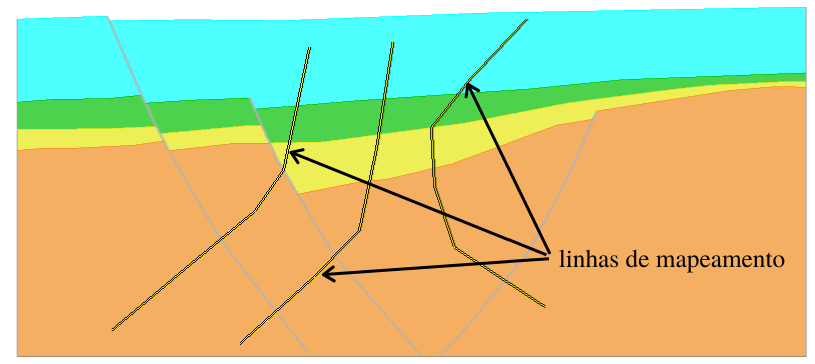
\includegraphics[width=\textwidth]{images/fig-linhas-de-mapeamento-ed}
    \caption{Linhas de mapeamento em uma seção.}\label{fig-linemap}
  \end{center}
\end{figure}

A Figura~\ref{fig-linemap-history} apresenta o resultado após uma transformação do tipo \textit{move sobre falha} (MSF)~\cite{Recon} onde é possível observar, além da deformação da camada, a linha de mapeamento sofrendo a mesma movimentação. Este tipo de uso pode ser interpretado como se houvesse ali um falso horizonte para avaliar o quantidade de movimento na restauração do rejeito.

\begin{figure} [h]
  \begin{center}
    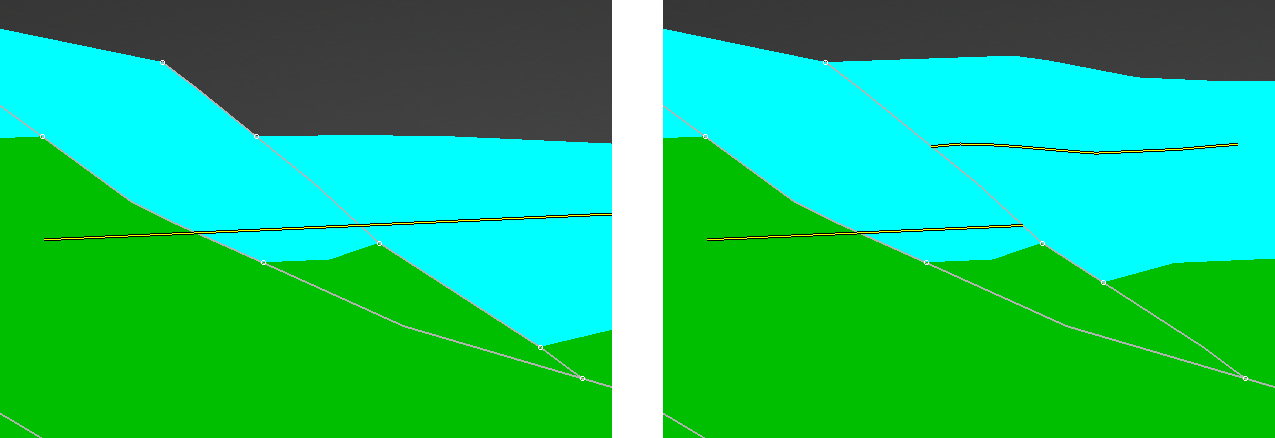
\includegraphics[width=\textwidth]{images/fig-linemap-history}
    \caption{Linhas de mapeamento em diferentes etapas}\label{fig-linemap-history}
  \end{center}
\end{figure}

\section{Criação das Linhas de Mapeamento}

O processo de criação da linha de mapeamento é feito para cada parte individualmente, de forma que, ao visualizar as partes tem-se a linha de mapeamento completa. Na Figura~\ref{fig-linemap-malhas} é possível ver uma linha de mapeamento cortando algumas regiões diferentes.

\begin{figure} [h]
  \begin{center}
    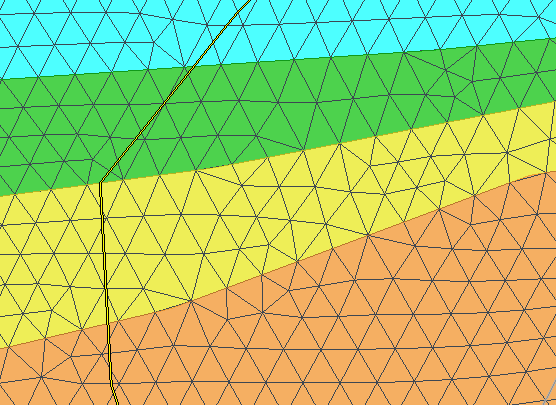
\includegraphics[width=250pt]{images/fig-linhas-de-mapeamento-malhas}
    \caption{Linhas de mapeamento cortando múltiplas faces.}\label{fig-linemap-malhas}
  \end{center}
\end{figure}

Na Figura~\ref{fig-linemap-parts} estão evidenciadas as partes que formam a linha de mapeamento. Como já dito, cada parte está associada à malha de um região diferente.

\begin{figure} [h]
  \begin{center}
    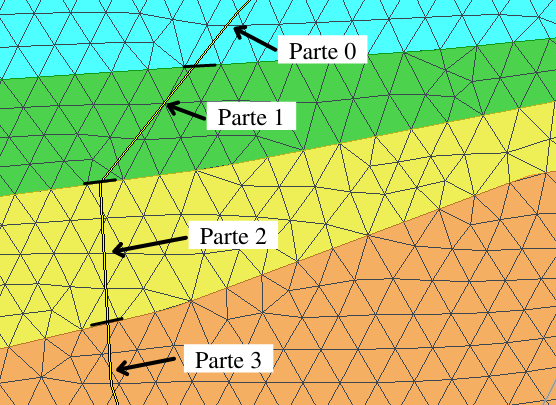
\includegraphics[width=250pt]{images/fig-lm-parts}
    \caption{Partes de uma linha de mapeamento}\label{fig-linemap-parts}
  \end{center}
\end{figure}

A Figura~\ref{fig-lm-topo} mostra a identificação dos pontos em uma parte de linha de mapeamento e a Tabela~\ref{tab-lm-topo} exibe quais informações topológicas são salvas de cada ponto.

\begin{figure} [hbt!]
  \begin{center}
    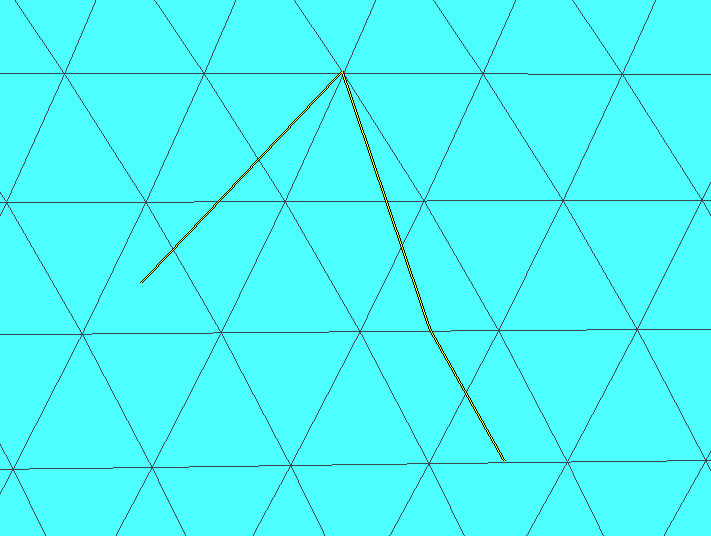
\includegraphics[width=260pt]{images/fig-lm-topo}
    \caption{Informações topológicas da malha mapeadas para a linha de mapeamento.}\label{fig-lm-topo}
  \end{center}
\end{figure}

% -*- coding: utf-8; -*-

\begin{table} [hbt!]
 \begin{center}
	 \caption{Informações topológicas salvas na linha de mapeamento.\label{tab-lm-topo}}
	~\\[-2mm]
	 \begin{tabularx}
		 {\textwidth}
		 {cp{2.0cm} lp{3.0cm} lp{10.0cm}}

		 \textbf{Ponto}
		 & \textbf{Tipo}
		 & \textbf{Informação armazenada} \\ \toprule

		 %~\\[-1mm]
		 A
		 & Elemento
		 & id=30, coordenadas baricêntricas=(0,33; 0,33; 0,33) \\ \midrule

		 %~\\[-1mm]
		 B
		 & Nó   
		 & id=431 \\ \midrule

		 %~\\[-1mm]
		 C
		 & Aresta
		 & id=130, coordenada paramétrica=0,45 \\ \midrule

		 %~\\[-1mm]
		 D
		 & Aresta
		 & id=145, coordenada paramétrica=0,55 \\ \midrule

	 \end{tabularx}
 \end{center}
\end{table}


\section{Derivações das Linhas de Mapeamento}

As linhas de mapeamento têm também casos de usos mais especializados dentro do Sistema Recon, como na criação e representação de poços. Poços são criados semelhantemente às linhas ou por importação de modelos com poços em 3D. Possuem característica de serem linhas quase verticalizadas e possuem uma finalidade mais limitada. Nos casos de poços 3D, a linha correspondente ao poço é apenas uma projeção do objeto tridimensional no plano da seção.

Há o uso nas chamadas linhas de interseção (\textit{CrossLine}) que servem para identificar e mapear as linhas de cruzamento entre seções no espaço tridimensional do multisseções, com isso é possível ter uma noção do que ocorre com seções transversais mesmo estando no domínio bidimensional da restauração.

Por último, foi criada a \textit{linha de mapeamento do modelo} ou \textit{LMModel}, cujo objetivo é servir para o mapeamento de linhas geológicas das seções para superfícies de horizontes geológicas e falhas. As \emph{LMModels} representam os elementos geológicos ao longo da restauração do modelo. Assim, é possível ter um acompanhamento do que ocorre com as entidades geológicas na seção, além de poder verificar como se deu a movimentação de cada ponto de horizonte, falha ou topo de sal ao longo da restauração.

As \textit{LMModels} são linhas de mapeamento baseadas no pontos do contorno da malha das regiões, ou seja, as partes que a formam possuem apenas pontos de mapeamento do tipo nó.

Pelo objetivo proposto, as \textit{LMModels} são linhas de mapeamento que tomam a geometria das entidades geológicas como entrada. Então, não há necessidade de criar uma linha-guia como é feita na linha de mapeamento original; a própria linha de horizonte, falha, ou topo de sal é usada como linha-guia.

Conforme o tipo do elemento geológico base, há um tipo de \textit{LMModel} e informações adicionais armazenadas:

\renewcommand{\labelitemi}{•}
\begin{itemize}
  \item Horizonte: é guardado a informação de idade deste horizonte.
  \item Falha: o identificador da falha é o dado armazenado.
  \item Topo de sal: apenas uma referência direta à linha original.
\end{itemize}

Todas essas informações  geológicas atreladas ao mapeamento topológico das \textit{LMModels}, quando em conjunto com as diversas seções geológicas de um modelo multisseções, são o que fazem dela o principal dado para a realização de um mapeamento de informações de evolução do modelo tridimensional ao longo do tempo, já que trazem todo o histórico de movimentação das camadas de um modelo geológico.

A maneira de trabalhar com \textit{LMModels} é com a organização delas em estruturas de dados que formam subconjuntos divididos por etapa de restauração e idade (caso de linhas de horizonte), o que é visto na sequência. Com isso, é obtido o conjunto de informações que representam a restauração das seções no Sistema Recon.

\begin{figure} [h]
  \begin{center}
    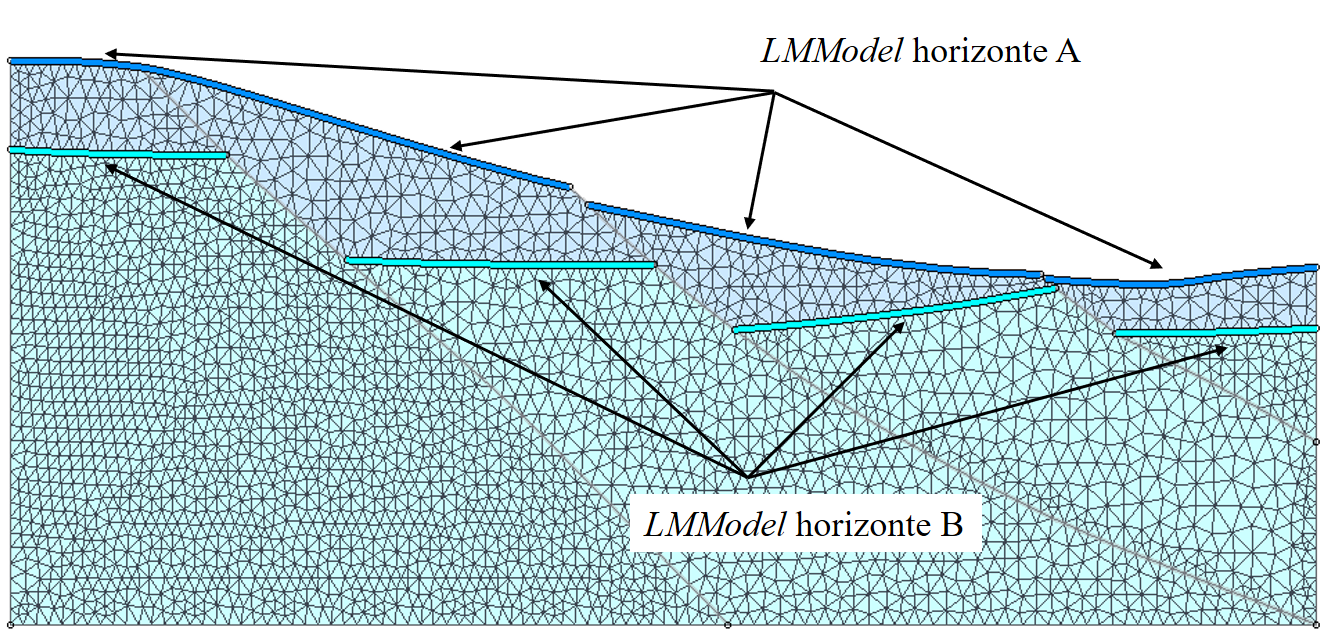
\includegraphics[width=350pt]{images/fig-lmmodel-example}
    \caption{\textit{LMModels} em uma seção geológica no Sistema Recon}\label{fig-lmmodel-example}
  \end{center}
\end{figure}

A Figura~\ref{fig-lmmodel-example} mostra \textit{LMModels} de dois horizontes diferentes. A representação delas dentro do Sistema Recon é feita com uma linha de maior espessura que as linhas de horizonte. No entanto, os pontos são os mesmos do contorno da malha. Observa-se na Figura~\ref{fig-lmmodel-mesh-diff} a diferença entre a linha de horizonte e a \textit{LMModel}, evidenciando o contorno da malha entre as duas regiões.

\begin{figure} [h!]
  \begin{center}
    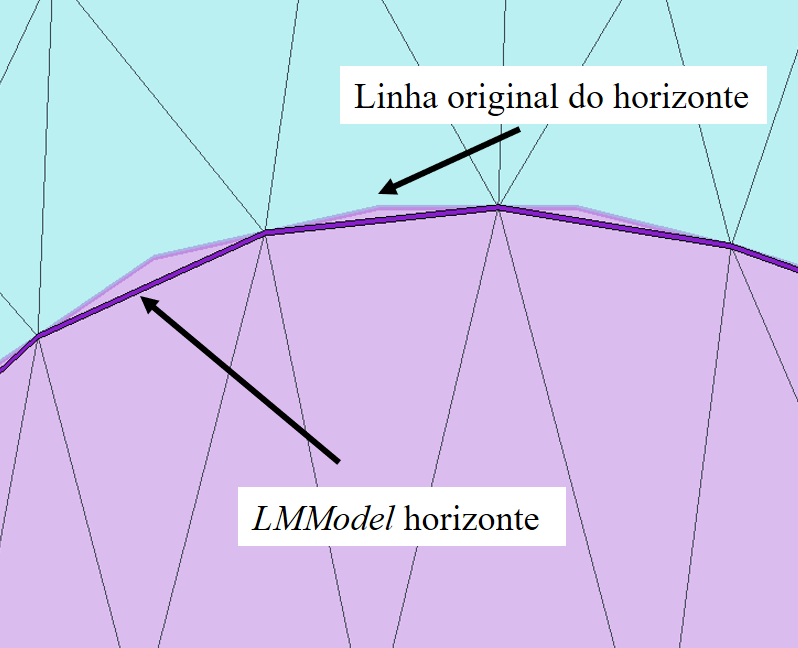
\includegraphics[width=275pt]{images/fig-lmmodel-mesh-diff}
    \caption{Diferença entre \textit{LMModel} e a linha de horizonte e uma seção geológica no Sistema Recon}\label{fig-lmmodel-mesh-diff}
  \end{center}
\end{figure}

A ilustração na Figura~\ref{fig-lmmodel-ms} apresenta as \textit{LMModels} de dois horizontes em um modelo multisseções. É esse conjunto de informações no ambiente tridimensional que será usado como parâmetro para o mapeamento de superfícies no Sistema Recon.

\begin{figure} [h!]
  \begin{center}
    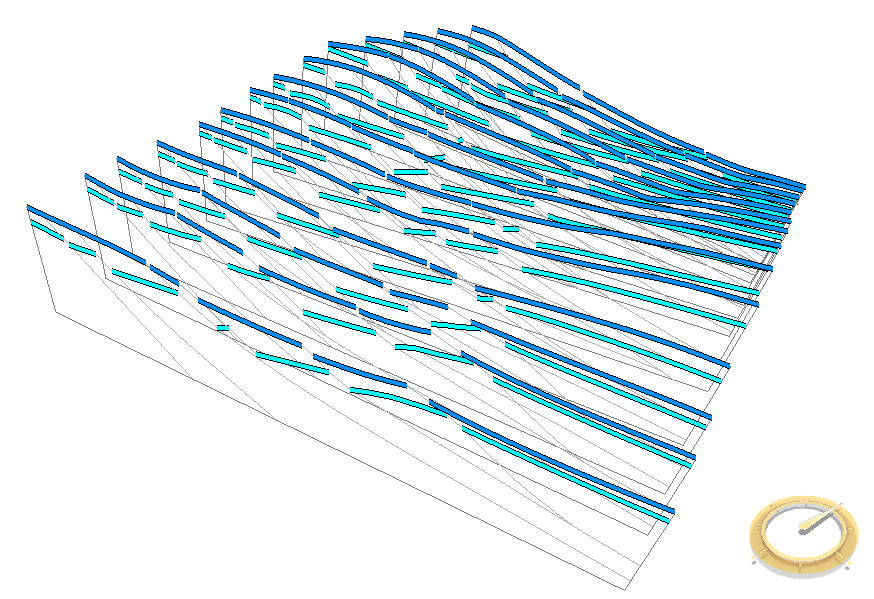
\includegraphics[width=300pt]{images/fig-lmmodel-ms}
    \caption{\textit{LMModels} no ambiente multisseções do Sistema Recon}\label{fig-lmmodel-ms}
  \end{center}
\end{figure}


